\documentclass[12pt]{article}
\usepackage{enumerate}
\usepackage[margin=1in]{geometry}
\usepackage{mathtools}
\usepackage{amsthm}
\usepackage{amsmath}
\usepackage{amssymb}
\usepackage{setspace,mathptmx}
\onehalfspacing

\usepackage{natbib}
\usepackage{tikz}
\usetikzlibrary{shapes}
\usepackage{amsmath}
\usepackage{xspace}
\newcommand{\A}{\ensuremath{\mathcal{A}}\xspace}
\newcommand{\B}{\ensuremath{\mathcal{B}}\xspace}
\newcommand\pa[1]{\ensuremath{\left(#1\right)}}

\usepackage{graphicx}
\usepackage{sidecap}
\usepackage{caption}
\usepackage {tikz}
\usepackage[utf8]{inputenc}
\usepackage{placeins}
\usepackage{threeparttable}
\usepackage{multirow}
\usepackage{rotating}
\usepackage[hidelinks]{hyperref}
\usepackage{textcomp}
\usepackage{tablefootnote}
%\usepackage{slashbox}
\usepackage{pifont}
\newcommand{\cmark}{\ding{51}}
\newcommand{\xmark}{\ding{55}}

\newtheorem{proposition}{Proposition}
\newtheorem{lemma}{Lemma}
\newtheorem {assumption}{Assumption}
\title{More Productive Under Preferred Incentives? \\ A Study on Performances With In/consistent Intrinsic And External Motives\footnote{Thanks to xxxx}}
%\author{Xiaogeng Xu and Fehime Ceren Ay\footnote{Address: Department of Economics, Norwegian School of Economics. Helleveien 30, 5045 Bergen Norway.}}

\begin{document}
\maketitle
\section{Introduction}
Incentives have impacts on performance. Recent research finds that people have different preferences in the incentives due to gender, beliefs and risk attitudes \citep{Niederle2007, Apicella2017}. With self-selection allowed, people would choose different incentive schemes to compensate their performances. Output also varies among different self-selected incentive schemes \citep{Dohmen2011a}. However, sometimes self-selection is not allowed and incentives are exogenously imposed. Some would then work under an incentive scheme that is inconsistent with their preferences. Given an incentive scheme, would people who self-select to the incentive perform better than those who prefer alternative incentives? Conditional on incentive preferences, would exogenous incentives make differences in performance? These questions are interesting in education, organizational management, as well as political institutions. This idea asks how the determination of incentives, self-selection or exogenous determination, influences performance, and whether the inconsistency of preferences and incentives has impacts on performance. 

%Examples: Among the attributes of intrinsic motivation, this project focuses on self determination. When people are given to the right to make a decision on own behalf, they may exert more efforts and show higher performance than when they are not given the right to decide. Empirically, we see that tax policy made by public voting may lead to less tax evasions. Also, companies with flatter hierarchy and more right given to employees may encounter less moral hazard than companies with steeper hierarchy. Similarly, children's performance of housework sometimes turns to be lower when they get paid than when they are not paid.

%Crowd-in/out effects: The performance, therefore, is influenced by both intrinsic motivation and external incentives. External incentives sometimes crowd in intrinsic motivations whereby the performance is enhanced. This crowd-in effects take place for some people so that the external incentives encourage them to exert more efforts thus higher performance. However, external incentives may crowd out intrinsic motivations. Thus, instead of motivating the external incentives discourage people and lower performance is observed compared to the performance in absence of the external incentives.

\section{Research questions}

There are three research questions. First, would self-selection of incentives bring better performance than exogenous assignment does?  Second, would exogenous incentives influence performances given preferences of incentives? Third, would preferences of incentives make performances different given an exogenous incentive?

\section{Related literature}

\citet{Gneezy2003} found that given indifferent inherent ability men's performance grows better when exogenous incentive changes from piece rate to tournament while women's performance is insensitive to the change of incentive (task: maze within 15 minutes, without self selection about incentive). \citet{Niederle2007} observed that men are twice likely to self select to tournament incentive and that performance in tournament incentive is higher than that in piece rate (task: add up five 2-digit numbers in 5 minutes). Also, they found that performance do not differ between those who enter and not enter tournament scheme. Similarly, \citet{Dohmen2011a} found no difference of performance among people self select into incentives of piece rate, tournament and revenue sharing (task: multiply 1-digit with 2-digit with five or ten minutes). And, the sorting is largely explained by productivity and risk attitudes. Whereas, \citet{Apicella2017} found that there is no gender difference when people compete against themselves whereas the performance is boosted by the self selected incentive. A recent paper by \citep{Quidt2017} showed that penalty contract leads to hight effort than bonus contract, which is explained by commitment instead of loss aversion or belief of performance. \citet{Mellizo2017} found out that when workers produce remarkably more when they have voice in choosing incentives then no voice. 

What distinguishes this idea from the existing papers is that this idea concerns about absolute own performance, instead of relative performance. Thus, competition or preference for competition is replaced with incentive that only depends on own performance in this idea. Unlike some papers above where both beliefs of own and others' performance are relevant, only belief of own performance is relevant in this context. The very difference is that this idea revolves around the effects of in/consistency between intrinsic preferences and external incentive on performance. Moreover, the effects of how the incentive is assigned on performance (e.g., self determined or externally assigned) is put in question, which is rarely seen to our best knowledge.

\section{Experiment design}

This experiment uses the task of adding up three 2-digit numbers (or multiply, maze, puzzle etc.). There are two incentive options: one is piece rate payment where participants get one point for each correct answer and zero point for wrong answer. The other incentive is reward/punishment payment where participants get some points for each correct answer and lose some points for each wrong answer. The gained and lost points in the reward/punishment payment will depend on average performance based on their beliefs. In the task, participants are given ten minutes during which problems are shown sequentially on the screen. Skipping is not allowed in the task and correctness is not informed until the end of this experiment. The indicator of performances is the number of correct answers within the ten minutes.

As shown in the Figure \ref{fig:fig1}, all participants first practice the add-up questions in five minutes. They will get the payment based on a tournament. Specifically, they will be randomly grouped with another two participants and the one with best performance will get an extra payment on top of show-up fee.

Second, participants will be asked about their beliefs of their performance in the first step. I.e., they need to guess the percentage of correct answers among questions they have answered. The guess closest to the true performance will be rewarded. In case of tie, all the closest guesses will be rewarded. These beliefs can be used to identify subjects' confidence levels, and to predict preferences for incentives. When the beliefs are revealed, the gained and lost points will be set according to the observed average belief of performance\footnote{Suppose $\hat{x}$ and $\hat{y}$ are estimated numbers of correct and wrong answers. Then belief of percentage of correct answers is $B=\frac{\hat{x}}{\hat{x}+\hat{y}}$. And a, b and c are respectively points in piece rate payment, points to gain and points to lose in reward/punishment payment. The condition to make the two incentives equivalent is that $a\hat{x}=b\hat{x}-c\hat{y}$. Together with the other two conditions: $a=1pt$ and $b=2c$, $b$ and $c$ are solved to be $b=\frac{2B}{3B-1}$ and $c=\frac{B}{3B-1}$.}.

Third, 67\% participants are randomly assigned to Treatment 1 and Treatment 2, the rest 33\% (or less) are assigned into Treatment 3. Participants in Treatment 1 and 2 will be asked preferences between the two incentive schemes, piece rate or punish-reward. In Treatment 3, participants will not be asked about preferences for incentive schemes. 

Fourth, participants will continue perform the task of adding up three two-digit numbers in given ten minutes. Participants in Treatment 1 will perform the task under their preferred incentives, piece rate or punish-reward. Participants in Treatment 2 will be randomly assigned one of the two incentive schemes with a 50/50 chance. Likewise, participants in Treatment 3 will be randomly assigned one of the two incentive schemes with a 50/50 chance.

Last, all participants will finish a follow-up survey. In the survey, they will go through a game of multiple price list in order to elicit their risk preferences. Together with elicited belief, the risk preferences will help explain selection of the payment method\footnote{\citet{Murad2016} found that confidence and risk attitudes are highly correlated and are both exhibition of intrinsic characteristics.} Besides, they will be asked about math score, gender, education, age, math enjoyment, competitiveness etc.

%The relation between risk attitudes and confidence has been investigated in gender - competition and psychological studies. Yet, these studies generally focused on relative confidence. This experiment differs from most of the studies with similar tasks (NV, GV etc.) by the fact that it is focusing on self-decision and performance not the competition. For that reason, we focus on the absolute confidence to observe subjects’ self evaluation and risk preferences.

\newpage
\begin{figure}[h!]
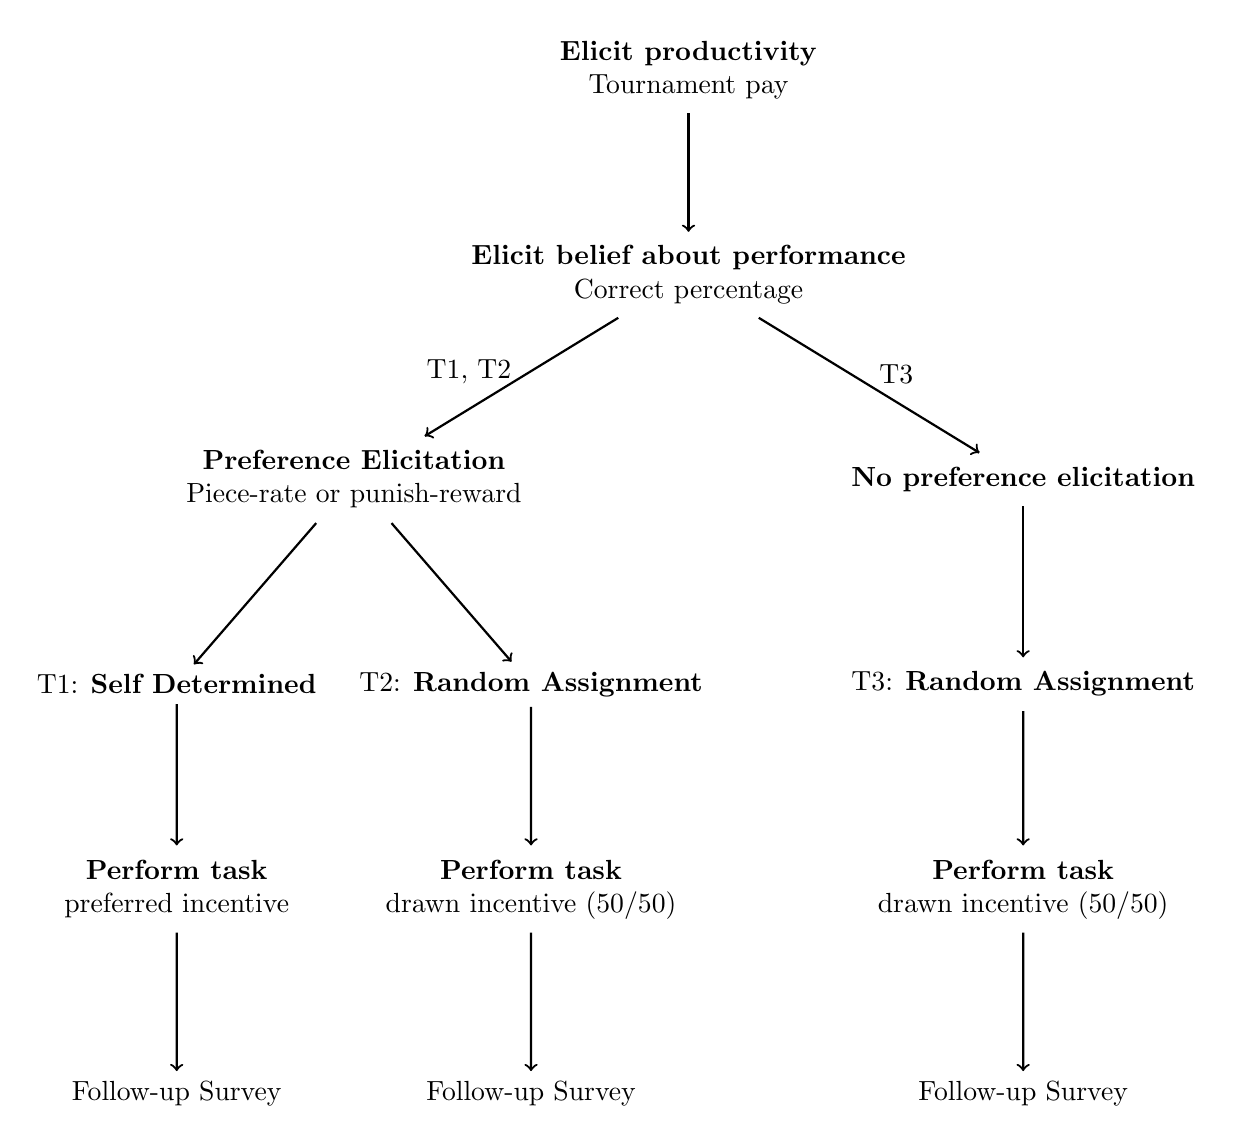
\begin{tikzpicture}
\node(0){\begin{tabular}{c}\textbf{Elicit productivity}\\Tournament pay\end{tabular}} [level distance=2.6cm, sibling distance=7cm]
child{node{\begin{tabular}{c}\textbf{Elicit belief about performance}\\Correct percentage\end{tabular}} [sibling distance=8.5cm] edge from parent [->, thick]
child{node{\begin{tabular}{c}\textbf{Preference Elicitation}\\ Piece-rate or punish-reward\end{tabular}} edge from parent [->, thick] 
[sibling distance=4.5cm]
child{node{T1: \textbf{Self Determined}}
child{node{\begin{tabular}{c}\textbf{Perform task}\\ preferred incentive\end{tabular}}
child{node{Follow-up Survey}}
}
}
child{node{T2: \textbf{Random Assignment}}
child{node{\begin{tabular}{c}\textbf{Perform task}\\ drawn incentive (50/50)\end{tabular}}
child{node{Follow-up Survey}}
}
}
edge from parent node[left, yshift=2]{T1, T2}
}
child{node{\begin{tabular}{c}\textbf{No preference elicitation}\end{tabular}} edge from parent [->,thick]
child{node{\begin{tabular}{c}T3: \textbf{Random Assignment}\end{tabular}} [sibling distance=5cm] edge from parent[->,thick]
child{node{\begin{tabular}{c}\textbf{Perform task}\\ drawn incentive (50/50)\end{tabular}}
child{node{Follow-up Survey}}
}
}
edge from parent node[right, yshift=4]{T3}
}
};
\end{tikzpicture}
\caption{Experiment procedure}
\label{fig:fig1}
\caption*{\small Note: Subjects first finish the task of two-digit plussing with tournament payment. Then their beliefs of performance will be elicited. These beliefs will determine the points setting of reward/punishment payment. In Treatment 1, participants are given the incentive they prefer. In Treatment 2, participants will be randomly given an incentive with a 50/50 chance. In Treatment 3, participants will be randomly given an incentive with a 50/50 chance. Piece rate payment is 1 point for each correct in ten minutes (E.g. 79+11+28=?). Reward/punishment means $b$ points for each correct and $c$ points for each wrong in ten minutes, where $b=\frac{2B}{3B-1}$ and $c=\frac{B}{3B-1}$ and $B$ is average belief of percentage of correct answers.}
\end{figure}

\section{Analysis}

As seen in Table \ref{tab:tab1}, the number of correct answers in the computing task is labeled as $Y$. The performances under the incentive piece rate is $Y^{s}$ and is $Y^{r}$ under the incentive punish-reward. If a participant prefers the piece rate to the punish-reward, the condition is written as $s\succ r$. Otherwise, the condition is $s\prec r$. Performances of participants in the three treatments are also included as a condition of the performances. Other covariates include productivity elicited in the first step, beliefs of performances, risk attitudes, gender, age, competitiveness and math enjoyment, etc. To test whether the source of incentives affects performances (research question 1), we need to compare performances with same preferences and incentives between Treatment 1 and Treatment 2.
\begin{equation*}\textit{source\,\,effects}=E[Y^{i}|i\succ j,\,\, T1]-E[Y^{i}|i\succ j,\,\, T2]\end{equation*}
where $i,\,\,j \in (s,\,\,r)$ and $i\neq j$.

To test the effects of incentives on performances (research question 2), we need to compare performances under different incentives within Treatment 2.
\begin{equation*}\textit{incentive\,\,effects}=E[Y^{i}|i\succ j,\,\,T2]-E[Y^{j}|i\succ j,\,\, T2]\end{equation*}
where $i,\,\,j \in (s,\,\,r)$ and $i\neq j$.

To test the effects of preferences on performances (research question 3), we need to compare performances with different preferences within Treatment 2.
\begin{equation*}\textit{preference\,\,effects}=E[Y^{i(j)}|i\succ j,\,\,T2]-E[Y^{i(j)}|j\succ i,\,\, T2]\end{equation*}
where $i,\,\,j \in (s,\,\,r)$ and $i\neq j$.

Since participants in Treatment 2 are asked about preferences prior to the task, the observed incentive effects and preference effects may be masked by lucky or unlucky feelings resulting from the resolution of the random assignment. Thus, by comparing performances between Treatment 2 and Treatment 3, the impacts of luck concern on performances will be manifested and the observed differences in the last two effects will be free of the luck concern which is caused by the preference elicitation. 

\begin{table}[]
\centering
\caption{Performances under incentives and preferences}
\label{tab:tab1}
\begin{tabular}{lrrr}
\hline
\textbf{Incentives}  & \multicolumn{2}{c} {\textbf{Preferences}}\\
                      & Piece rate (safe) & Punish reward (risky)\\\hline
T1 Self-determined       & $Y^{s}|s\succ r, T1$           & $Y^{r}|r\succ s, T1$         \\\hline
T2 Piece rate    & $Y^{s}|s\succ r, T2$            & $Y^{s}|r\succ s, T2$                            \\
T2 Punish reward & $Y^{r}|s\succ r, T2$            & $Y^{r}|r\succ s, T2$                            \\\hline
T3 Piece rate   & $Y^{s}|s\succ r, T3$             & $Y^{s}|r\succ s, T3$             \\
T3 Punish reward  & $Y^{r}|s\succ r, T3$       & $Y^{r}|r\succ s, T3$           \\\hline
\end{tabular}
\end{table}

\newpage
\bibliographystyle{../paper/bst/standard2}
\bibliography{../paper/bib/mmref}

\end{document}